\documentclass[12pt]{article}

\usepackage[margin=1in]{geometry}
\usepackage{tikz}
\usepackage{indentfirst}
\usepackage{setspace}

\usetikzlibrary{calc}
\usetikzlibrary{decorations.pathreplacing}

\title{Economics graphs}
\author{Andrew}
\date{\today}

\begin{document}
\setstretch{1.3}

Price for oil is at its lowest after a jump in supply and signs of steadily decreasing demand. In response, OPEC has cut their supply in hopes to increase their total revenue. However, their actions are debatable: are the cuts beneficial or detrimental? \\

Demand is the various quantities of a good or service that consumers are willing and able to purchase at various prices. On the contrary, supply refers to the various quantities that suppliers are willing and able to produce at various prices. Furthermore, price elasticity of demand (PED) is the ratio of percentage change in quantity demanded to percentage change in price. PED gauges how responsive consumers are to a change in price.


%%%						GRAPH 1						%%%

\begin{center}
\ \ \ \ \ Figure 1. Market for Oil

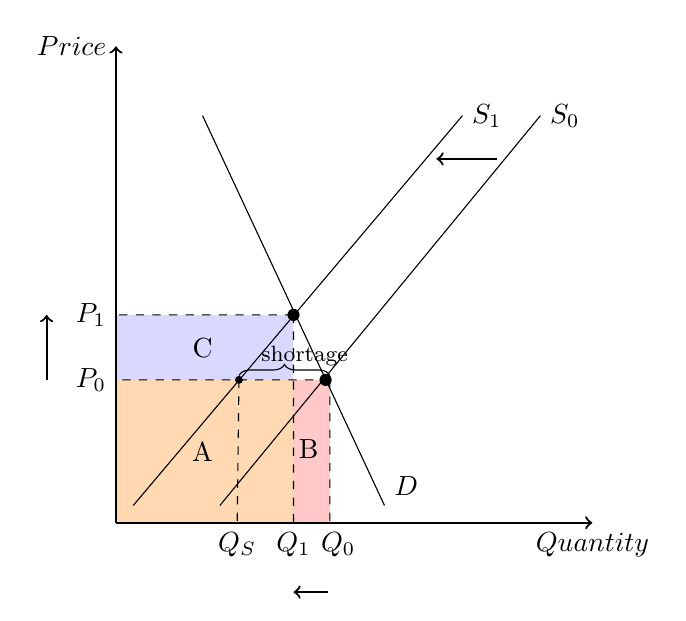
\begin{tikzpicture}[scale= 1.1]

% Define coordinates.

	%axes

	\coordinate (origin) at (0,0);
	\coordinate [label= left:$Price$] (P) at (0, 5.5);
	\coordinate [label= below:$Quantity$] (Q) at (5.5, 0);
	
	%demand curve
	\coordinate (demandTail) at (1, 4.7);
	\coordinate [label= above right:$D$] (D) at (3.1, 0.2);
	
	%supply curve 1
	\coordinate (supplyTail1) at (0.2, 0.2);
	\coordinate [label= right:$S_1$] (S) at (4, 4.7);
	
	%supply curve 0 
	\coordinate (supplyTail0) at (1.2, 0.2);
	\coordinate [label = right:$S_0$] (S0) at (4.9, 4.7);
	
	%Equilibria 
	\coordinate (E1) at (2.05, 2.4);	
	\coordinate (E2) at (2.47, 1.65);
	
% Colour in.

	\fill [fill=orange!30] (0, 0) -- (0, 1.65) -- (2.05, 1.65) -- (2.05, 0) -- cycle;
	
	\fill [fill=blue!15!white] (0, 1.65) -- (0, 2.4) -- (2.05, 2.4) -- (2.05, 1.65) -- cycle;
	
	\fill [fill=red!21!white] (2.05, 0) rectangle (2.47, 1.65);

	 
% Draw axes.

	\draw[thick, ->] (origin) -- (P);
	\draw[thick, ->] (origin) -- (Q);  
	
% Draw lines.
		
	\draw (demandTail) -- (D);
	\draw (supplyTail1) -- (S);
	\draw (supplyTail0) -- (S0);
	
	\draw[dashed] (E1) -- (2.05, 0) node[below] {$Q_1$};
	\draw[dashed] (E1) -- (0, 2.4) node[left] {$P_1$};
	
	\draw[dashed] (E2) -- (2.47, 0) node[below, xshift=3pt] {$Q_0$};
	\draw[dashed] (E2) -- (0, 1.65) node[left] {$P_0$};
	
	\draw[dashed] ($(E2) + (-1.05, 0)$) -- (1.4, 0) node[below] {$Q_S$};
	
	\draw[thick, ->]($(S0) + (-0.5, -0.5)$) -- ($(S) + (-0.3, -0.5)$);
	
% Draw area labels.

	\draw (1, 0.6) node[above]{A};
	\draw (1, 1.8) node[above]{C};
	\draw (2, 0.85) node[right] {B};
	
% Draw points of equilibria. 

	\fill[black] (E1) circle (2pt);
	\fill[black] ($(E2) + (-0.05,0)$) circle (2pt);
	
	\fill[black] ($(E2) + (-1.05, 0)$) circle (1.3pt);
	
% Draw label arrows.

	\draw[thick, ->] (-0.8, 1.65) -- (-0.8,2.4);
	\draw[thick, ->] (2.45, -0.8) -- (2.05, -0.8);
	
	
	\draw [decorate, decoration ={brace,amplitude=4pt},xshift=-4pt,yshift=0pt] ($(E2) + (-1.05, 0.05)$) -- ($(E2)+ (0, 0.05)$) node [above left,xshift=10pt] {\footnotesize shortage}; 

\end{tikzpicture}

\end{center}



Figure 1 illustrates the effect of OPEC limiting supply on total revenue, though it holds demand constant. Given that oil is a good that is price inelastic in demand because it has few substitutes and is essentially a necessity, increased total revenue could be achieved by increasing price. The increase in price would be proportionately greater than the decrease in quantity demanded because of oil's relatively low  PED. OPEC’s attempt to maintain the price of oil by decreasing the supply of oil, is illustrated in Figure 1 as a leftward shift of the supply curve from  $S_0$ to $S_1$. Note that in Figure 1, total revenue, before the decrease in supply, is represented as the rectangle with vertices $P_0$ and $Q_0$: area  $A + B$. After the production cuts, total revenue becomes the rectangle with vertices $P_1$ and $Q_1$: area $A + C$. After the market adjusts from the shortage of  $Q_0 - Q_S$  units, the market equilibrium price increases to $P_1$, while equilibrium quantity decreases to  $Q_1$. Therefore, OPEC's strategy to cut oil production can theoretically increase total revenue.


\newpage


%%%						GRAPH 2						%%%			

\begin{center}

\ \ \ \ \ Figure 2. Market for Oil

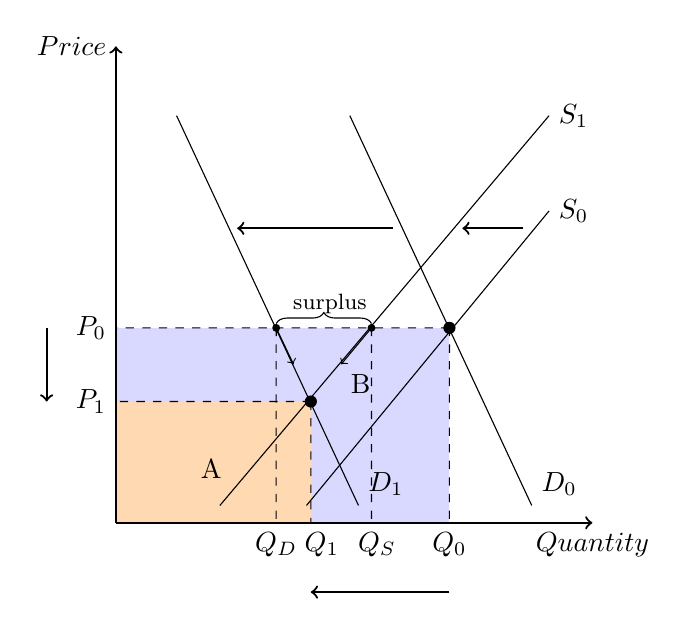
\begin{tikzpicture}[scale= 1.1]

% Define coordinates.

	%axes

	\coordinate (origin) at (0,0);
	\coordinate [label= left:$Price$] (P) at (0, 5.5);
	\coordinate [label= below:$Quantity$] (Q) at (5.5, 0);
	
	%demand curve 1
	\coordinate (demandTail) at (0.7, 4.7);
	\coordinate [label= above right:$D_1$] (D) at (2.8, 0.2);
	
	%demand curve 0
	\coordinate (demandTail0) at (2.7, 4.7);
	\coordinate [label= above right:$D_0$] (D0) at (4.8, 0.2);
	
	%supply curve 1
	\coordinate (supplyTail1) at (1.2, 0.2);
	\coordinate [label= right:$S_1$] (S) at (5, 4.7);
	
	%supply curve 0 
	\coordinate (supplyTail0) at (2.2, 0.2);
	\coordinate [label = right:$S_0$] (S0) at (5, 3.6);
	
	%Equilibria 
	\coordinate (E1) at (3.85, 2.25);	
	\coordinate (E2) at (2.25, 1.4);
	
	\coordinate (X) at (2.95, 2.25);
	\coordinate (Y) at (1.85, 2.25);
	
% Colour in.

	\fill [fill=blue!15!white] (0,0) rectangle (E1);
	\fill [fill=orange!30] (0, 0) rectangle (E2);
	 
% Draw axes.

	\draw[thick, ->] (origin) -- (P);
	\draw[thick, ->] (origin) -- (Q);  
	
% Draw lines.

	\draw (demandTail0) -- (D0);		
	\draw (demandTail) -- (D)node[above right] {$D_1$};
	\draw (supplyTail1) -- (S);
	\draw (supplyTail0) -- (S0);
	
	\draw[dashed] (E1) -- (3.85, 0) node[below] {$Q_0$};
	\draw[dashed] (E1) -- (0, 2.25) node[left] {$P_0$};
	
	\draw[dashed] (E2) -- (2.25, 0) node[below, xshift=4pt] {$Q_1$};
	\draw[dashed] (E2) -- (0, 1.4) node[left] {$P_1$};
	
	\draw[dashed] (X) -- (2.95, 0) node[below, xshift=2pt] {$Q_S$};	
	\draw[dashed] (Y) -- (1.85, 0) node[below] {$Q_D$};
	
	\draw[thick, ->](4.7, 3.4) -- (4, 3.4);
	\draw[thick, ->](3.2, 3.4) -- (1.4, 3.4);
	
	\draw[->] (Y) -- (2.05, 1.83);
	\draw[->] (X) -- (2.6, 1.83);
	
% Draw area labels.

	\draw (1.1, 0.4) node[above]{A};
	\draw (2.6, 1.6) node[right]{B};
	
% Draw label arrows.

	\draw[thick, ->] (-0.8, 2.25) -- (-0.8, 1.4); 
	\draw[thick, ->] (3.85, -0.8) -- (2.25, -0.8);

% Draw equlibria.

	\fill[black] (E1) circle (2pt);
	\fill[black] (E2) circle (2pt);
	
	\fill[black] (X) circle (1.3pt);
	\fill[black] (Y) circle (1.3pt);
	
		\draw [decorate, decoration ={brace,amplitude=4pt},xshift=-4pt,yshift=0pt] ($(Y) + (0, 0.05)$) -- ($(X) + (0, 0.05)$) node [above, xshift=-15pt] {\footnotesize surplus}; 


\end{tikzpicture}
\end{center} 

Figure 2 illustrates how the scenario actually played out. A deteriorating global economy kept demand low enough so that despite OPEC's production cuts, prices were still able to fall. Consumers started to lose buying power and therefore were not as willing to consume as much oil. This can be illustrated as a leftward shift in the demand curve from  $D_0$  to  $D_1$ . Additionally, after OPEC cut oil production, supply decreased. This is represented as a leftward shift of the supply curve from  $S_0$  to  $S_1$ . However, despite OPEC's attempts to raise total revenue by cutting production by 520 000 barrels, prices still fell. We can deduce that this was because the relative magnitude of the shift left of the demand curve was greater than that of the shift left of the supply curve. Furthermore, a reduction in total revenue is shown in the revenue rectangles. Before the decreases in supply and demand, total revenue is illustrated as area $A + B$ (the rectangle with vertices $P_0$  and  $Q_0$). After the decreases, total revenue is pictured as area $A$, which is clearly less than $A + B$.\\

OPEC’s intention to cut production in order to raise total revenue was questionable. Yes, given that increased total revenue in the market for oil, would also increase government indirect tax revenues around the world since business would fare better. This would mean that more money would be available to spend on healthcare and infrastructure, which we value as a society.  However, as seen in Figure 1, cutting supply, while holding demand constant, increases the price of oil, while decreasing its quantity traded. This is bad news for consumers, since oil is essentially a necessity because it has few substitutes. Thus, in the perspective of consumers, OPEC’s strategy was damaging. Although, given enough time, future technology may allow consumers to rely less on oil, diminishing the effects of similar situations that limit the availability of oil. \\

 A recession is defined as a significant decline in economic activity, across the economy. Given that when OPEC decided to cut production, there was a prevailing recession, we can argue that reducing production, and consequently, consumption of oil, in turn reduced economic activity. Reducing economic activity in the midst of a recession is not an effective solution.\\

Moreover, since demand was dwindling as a result of a deteriorating global economy, OPEC’s strategy failed to increase total revenue, while reducing the quantity traded of oil, as seen in Figure 2. Though, it should be noted that this was favourable for consumers, since falling oil prices weighed on pump prices.


\end{document}